\chapter{Schematy elektroniczne urządzeń}
\label{schematics}

\section{Urządzenie lokalizujące}
Ze względu na poziom skomplikowania układu, schemat elektroniczny musiał zostać rozbity na podschematy. W urządzeniu lokalizującym można wyróżnić trzy znaczące moduły elektroniczne, realizujące odpowiednie funkcje. Są to:

\begin{itemize}
\item Moduł zasilania, przedstawiony na rysunku \ref{fig:image_mainboard_power_schematic}
\item Moduł funkcjonalny, przedstawiony na rysunku \ref{fig:image_mainboard_functional_schematic}
\item Moduł NFC, przedstawiony na rysunku \ref{fig:image_mainboard_NFC_schematic}
\end{itemize}

\begin{figure}[H]
	\centering
	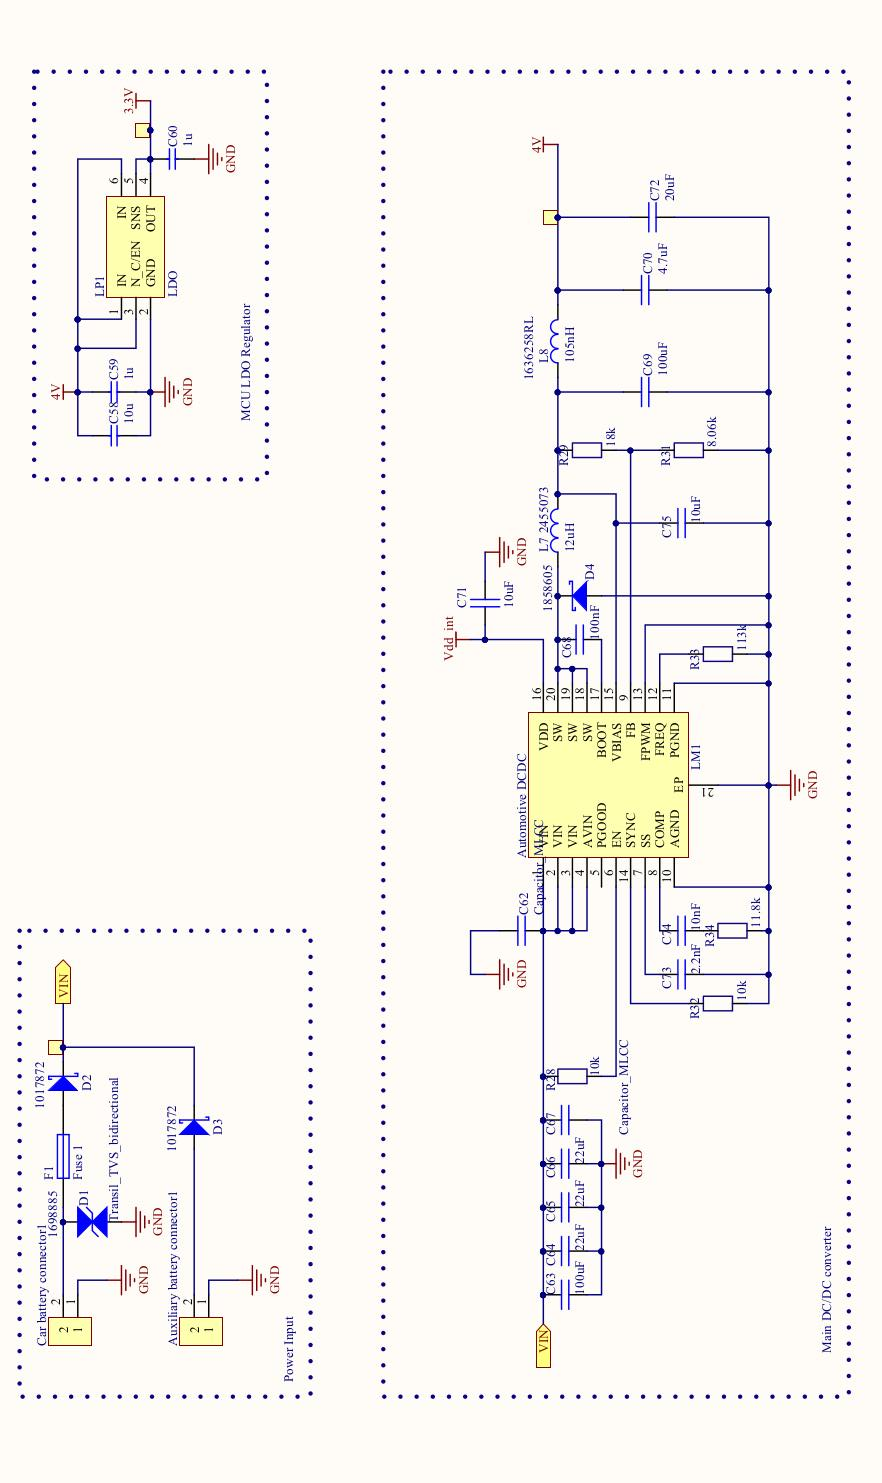
\includegraphics[width=14cm]{img/schematics/mainboard_power.jpg}
	\caption{Schemat modułu zasilania urządzenia lokalizującego}
	\label{fig:image_mainboard_power_schematic}
\end{figure}

\begin{figure}[H]
	\centering
	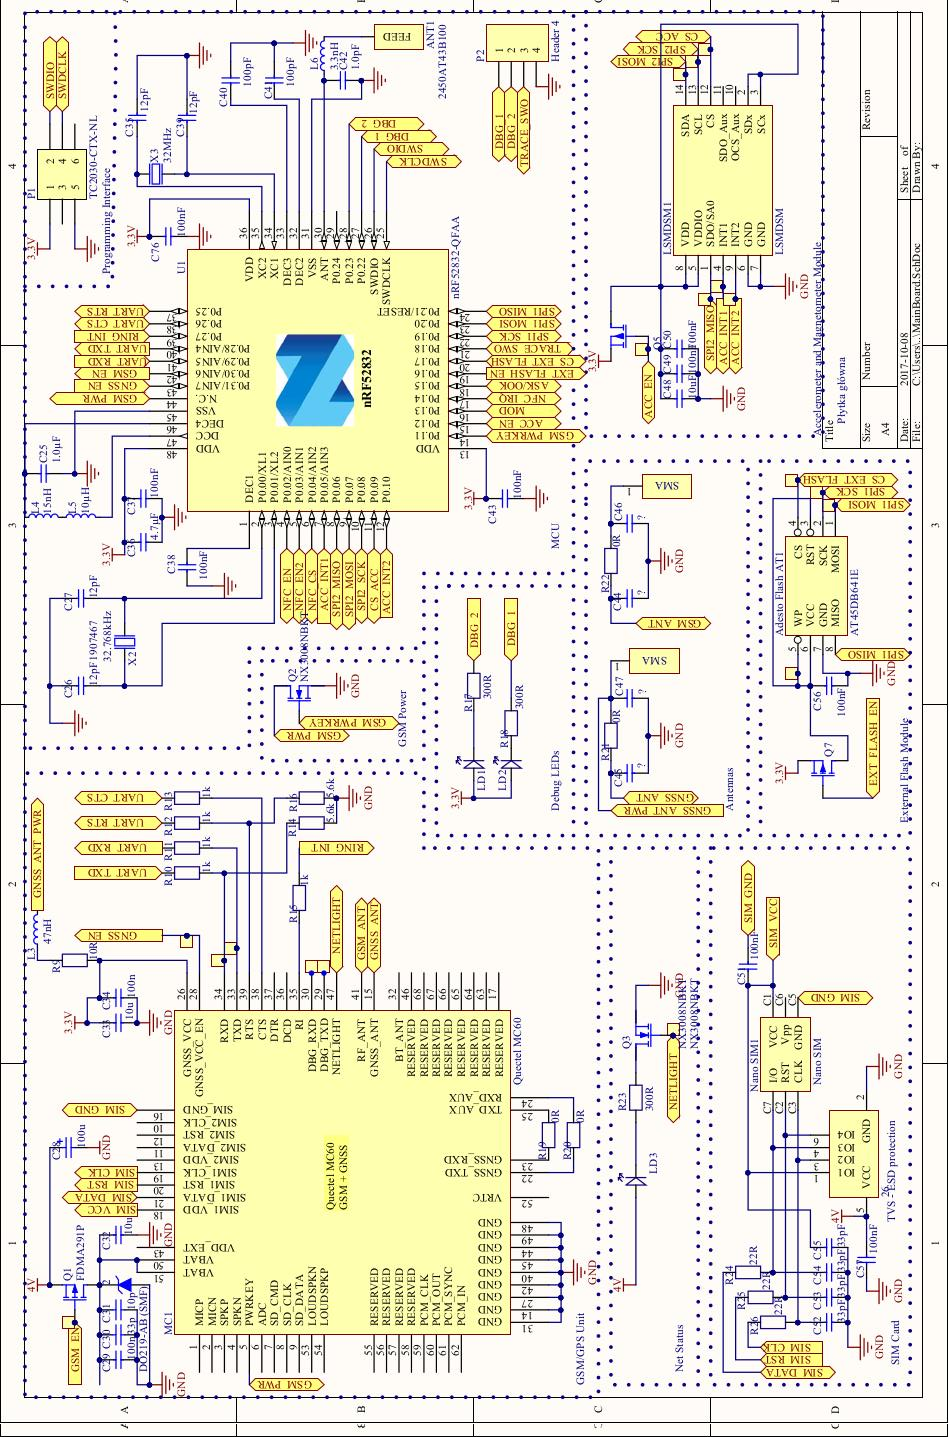
\includegraphics[width=14cm]{img/schematics/mainboard_functional.jpg}
	\caption{Schemat modułu funkcjonalnego urządzenia lokalizującego}
	\label{fig:image_mainboard_functional_schematic}
\end{figure}

\begin{figure}[H]
	\centering
	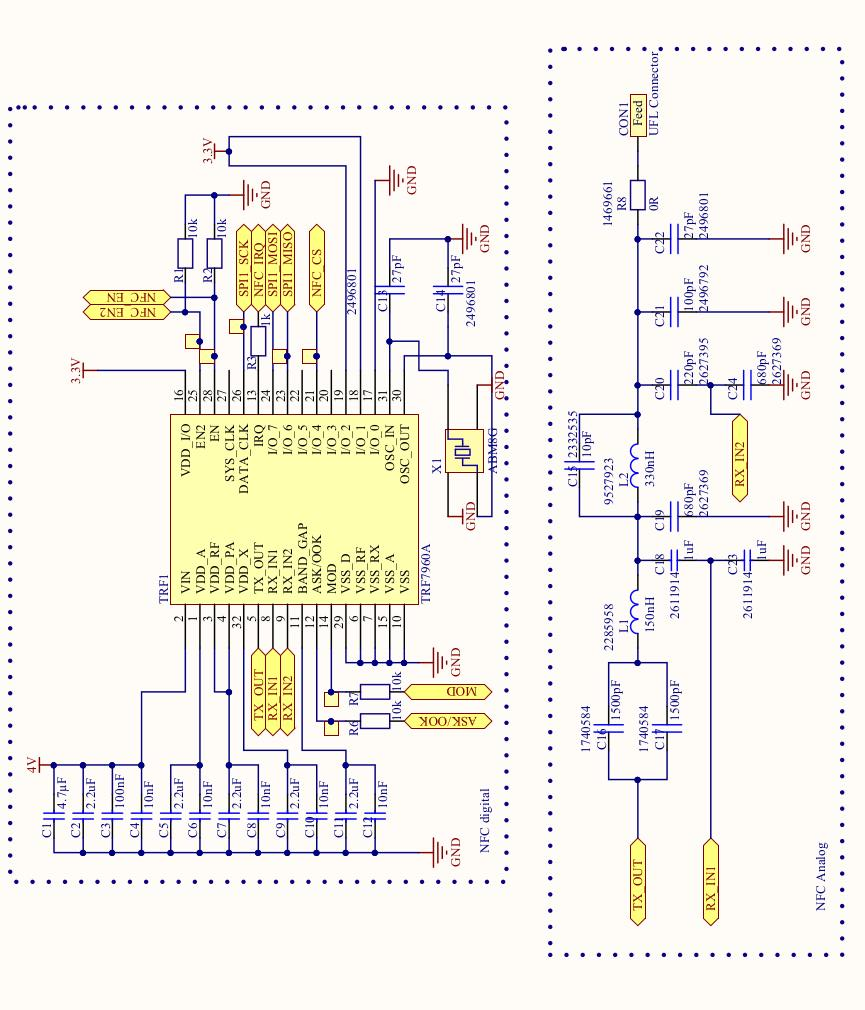
\includegraphics[width=14cm]{img/schematics/mainboard_NFC.jpg}
	\caption{Schemat modułu NFC urządzenia lokalizującego}
	\label{fig:image_mainboard_NFC_schematic}
\end{figure}



\subsection{Schemat zasilania}

Akumulator samochodowy jest bardzo wygodnym źródłem zasilania układów elektronicznych, lecz gdy są one niewłaściwie zaprojektowane, bywa on dla nich zabójczy. Bliska odległość do alternatora i innych urządzeń indukcyjnych powoduje generowanie silnych zakłóceń na linii zasilającej. Niekiedy "szpilki" napięciowe osiągają wartość rzędu 100V. Z tego powodu należy stosować transile – diody zabezpieczające. Powodują one ograniczenie zbyt dużego napięcia do pewnej maksymalnej wartości. W przypadku zastosowanego przeze mnie komponentu wynosi ono 24.4V. Zabezpieczenie przeciążeniowe stanowi bezpiecznik samochodowy o wartości 4A. 
Ponieważ jednym z wymagań układu jest możliwość zasilania bateryjnego, konieczne jest zastosowanie dodatkowego przyłącza zasilania. Urządzenie można zasilić dowolną baterią o napięciu od 4 do 38V i wydajności prądowej co najmniej 3A w szczycie. Ze względu na prawdopodobieństwo wystąpienia różnic napięć pomiędzy dodatkowa baterią, a akumulatorem samochodu i wiążącym się z tym przepływem prądu z jednego źródła do drugiego, konieczne jest zastosowanie diód zabezpieczających przed rozładowaniem baterii przez akumulator (gdy napięcie akumulatora niższe niż napięcie baterii) lub mogącym doprowadzić baterię do zniszczenia doładowywaniem jej bezpośrednio z akumulatora (gdy napięcie baterii jest od niższe napięcia akumulatora). W trakcie projektowania, zdecydowano się na zastosowanie diód Schottky’ego ze względu na ich niski spadek napięcia (0.2 - 0.55V w zależności od natężenia prądu) oraz szybki czas przełączania ze stanu zaporowego do przewodzenia (ograniczenie krótkotrwałych zaników zasilania przy wyłączaniu samochodu). Na rysunku \ref{fig:image_mainboard_power_input} przedstawiono część wejściową dla zasilania całej płytki.

\begin{figure}[H]
	\centering
	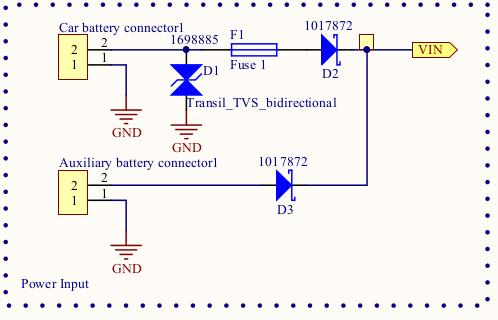
\includegraphics[width=10cm]{img/schematics/mainboard_power_input.jpg}
	\caption{Schemat modułu zasilania wejściowego urządzenia lokalizującego}
	\label{fig:image_mainboard_power_input}
\end{figure}

Niestety, często napięcie wejściowe, nawet po zadziałaniu zabezpieczenia w postaci transila, jest nadal zbyt duże dla zwykłych układów zasilających. Stąd konieczne jest stosowanie przetwornic impulsowych klasy automotive, które umożliwiają zasilanie napięciem wejściowym do kilkudziesięciu woltów. Schemat wykorzystanej przetwornicy przedstawiono na rysunku \ref{fig:image_mainboard_power_converter}.

\begin{figure}[H]
	\centering
	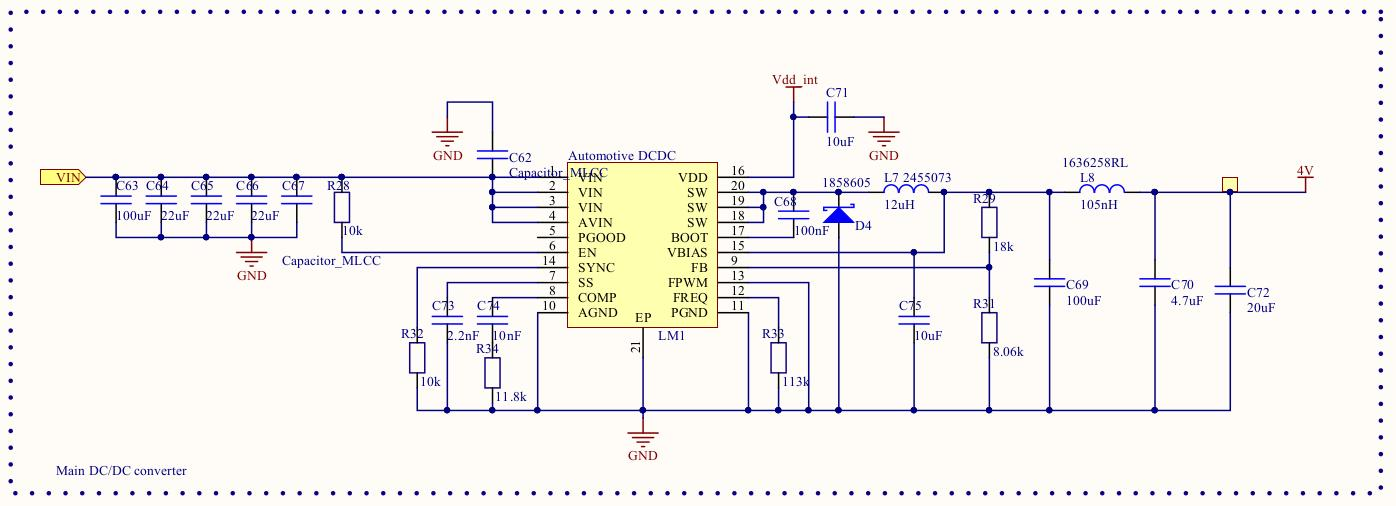
\includegraphics[width=17cm]{img/schematics/mainboard_power_converter.jpg}
	\caption{Schemat przetwornicy impulsowej modułu zasilania urządzenia lokalizującego}
	\label{fig:image_mainboard_power_converter}
\end{figure}

Zastosowana w urządzeniu przetwornica umożliwia zasilanie napięciami od 4 do 38V. Wybrano ją ze względu na niewielką liczbę zewnętrznych komponentów, niezbędnych do jej działania w porównaniu do innych modułów, a także wysoką sprawność rzędu od 85\% do 90\% w zależności od chwilowego natężenia prądu. Wytwarza ona na wyjściu napięcie o wartości 4V, którym zasilany jest moduł GSM oraz dalszy stopień obniżania napięcia.

Ostatni stopień zasilania generuje z napięcia wyjściowego z przetwornicy napięcie o wartości 3.3V. Jest ono niezbędne do zasilania układów mikrokontrolera, pamięci flash, akcelerometru oraz układu GPS. Szacowany pobór prądu przez te układy wynosi ok. 200mA w szczycie, stąd dla bezpieczeństwa wykorzystano stabilizator napięcia LDO (ang. Low Dropout Stabilizer) o maksymalnym natężeniu wyjściowym 0,5A. Jego schemat przdstawiono na rysunku \ref{fig:image_mainboard_power_ldo}.

\begin{figure}[H]
	\centering
	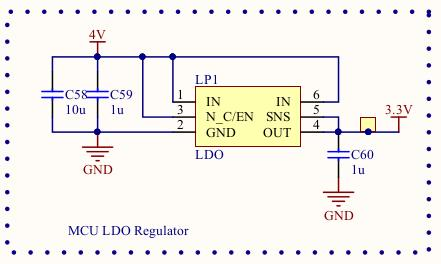
\includegraphics[width=12cm]{img/schematics/mainboard_power_ldo.jpg}
	\caption{Schemat stabilizatora napięcia modułu zasilania urządzenia lokalizującego}
	\label{fig:image_mainboard_power_ldo}
\end{figure}

\subsection{Moduł mikrokontrolera}

Serce urządzenia stanowi mikrokontroler nRF52832 firmy Nordic Semiconductor. Układ ten posiada 32 bitowy rdzeń Cortex-M4 zaprojektowany przez firmę ARM, sprzętową jednostkę FPU oraz 512kB wewnętrznej pamięci Flash oraz 64kB pamięci RAM. Zdecydowano się na wykorzystanie tego mikrokontrolera ze względu na kilka czynników. Pierwszym z nich jest jego wyposażenie- posiada wbudowany układ radiowy działający na częstotliwości 2.4 GHz i umożliwiający komunikację w standardzie Bluetooth Low Energy, ANT lub wykorzystanie własnego protokołu. Dodatkowym atutem tego mikrokontrolera jest wyposażenie w sprzętowy interfejs NFCT, umożliwiający wykorzystanie modułu jako tag (urządzenie podrzędne) w komunikacji poprzez interfejs NFC. Ponadto ma bardzo duże możliwości obliczeniowe – wewnętrzny zegar 64 MHz umożliwia bardzo szybkie wykonywanie zaprogramowanych zadań i szybki powrót do trybu oszczędzania energii. Zużycie energii przez ten procesor jest bardzo niewielkie. W trakcie wykonywania programu pobór prądu wynosi 58 $\mu A$ /MHz gdy kod wykonywany jest z pamięci flash, natomiast w trybie oszczędzania energii pobór spada do ok 1.9 $\mu A$. Ostatnim i być może najważniejszym czynnikiem decydującym na wybranie tego układu jest posiadane przez autora doświadczenie zawodowe w programowaniu układów od tego producenta, a zatem bardzo dobra znajomość jego możliwości i SDK (ang. Software Development Kit). Schemat mikrokontrolera przedstawiono na rysunku \ref{fig:image_mainboard_functional_mcu}.

\begin{figure}[H]
	\centering
	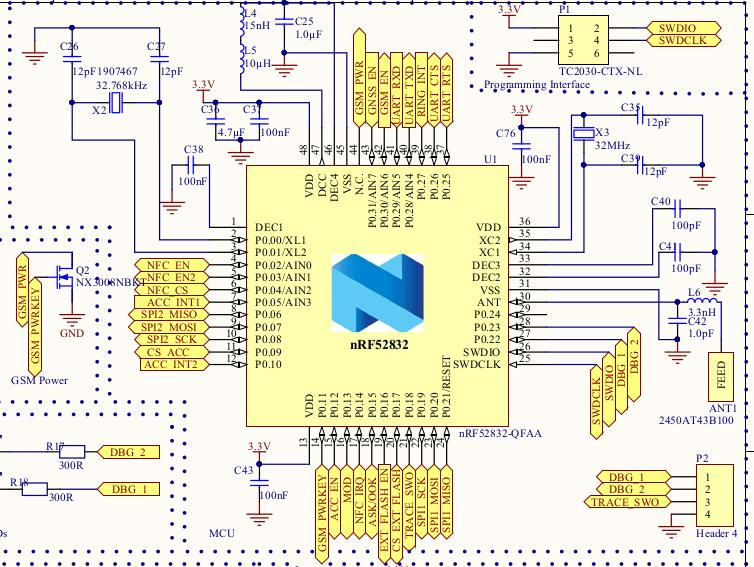
\includegraphics[width=15cm]{img/schematics/mainboard_functional_mcu.jpg}
	\caption{Schemat modułu mikrokontrolera w urządzeniu lokalizującym}
	\label{fig:image_mainboard_functional_mcu}
\end{figure}

\subsection{Moduł GSM i GPS}

Jako moduł realizujący główną funkcję urządzenia wybrano układ Quectel MC60. Stanowi on połączenie modułu GSM oraz GPS w jednym chipie. Umożliwia transmisję w wielu protokołach, takich jak: TCP/IP, UDP, FTP, PPP, HTTP czy NTP. Ponadto możliwe jest odbieranie danych w postaci krótkich wiadomości SMS. Układ posiada niewielkie wymiary: 18.7 mm x 16 mm x 2.1 mm dzięki czemu możliwe będzie zmniejszenie całego urządzenia. Zużycie energii wynosi:
\begin{itemize}
\item Około 25 mA gdy działa jedynie moduł GPS
\item Do 1.6 A w trakcie transmisji danych poprzez sieć GSM
\end{itemize}

Ponadto, kombinacja tych dwóch systemów umożliwia wykorzystanie funkcjonalności AGPS. Polega ona na podaniu do modułu GPS zgrubnych danych o położeniu satelitów, pobranych z sieci GSM. Dzięki temu, ustalenie własnej lokalizacji, nawet po długotrwałym wyłączeniu, trwa ok. sekundy (tzw. warm start). Schemat modułu GSM i GPS przedstawiono na rysunku \ref{fig:image_mainboard_functional_gps_gsm}.

\begin{figure}[H]
	\centering
	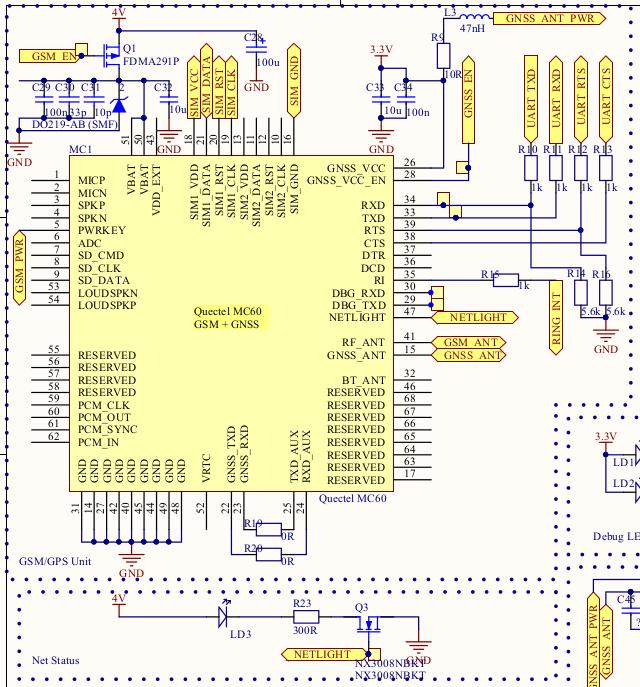
\includegraphics[width=15cm]{img/schematics/mainboard_functional_gps.jpg}
	\caption{Schemat modułu układu GSM i GPS w urządzeniu lokalizującym}
	\label{fig:image_mainboard_functional_gps_gsm}
\end{figure}

W celu zwiększenia niezawodności działania urządzenia, zdecydowano zastosować zewnętrzne anteny GSM i GPS poprawiające jakość sygnału. Dodatkowo, w celu zwiększenia jakości sygnału, antena GPS jest anteną aktywną. Oznacza to, że dostarczane jest do niej dodatkowe zasilanie, co powoduje wzmocnienie odebranego sygnału. Schemat anten przedstawiono na rysunku \ref{fig:image_mainboard_functional_gps_gsm_antennas}. Zawarte na nim znaki zapytania, zamiast wartości kondensatorów oznaczają, że kondensatory należy dobrać po złożeniu płytki i przebadaniu jej pod kątem jak najlepszego dopasowania impedancji.

\begin{figure}[H]
	\centering
	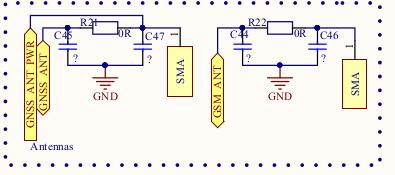
\includegraphics[width=15cm]{img/schematics/mainboard_functional_gps_gsm_antennas.jpg}
	\caption{Schemat modułu anten dla GSM i GPS w urządzeniu lokalizującym}
	\label{fig:image_mainboard_functional_gps_gsm_antennas}
\end{figure}

Ostatnią częścią układu GSM jest połączenie modułu z kartą SIM, umożliwiającą zalogowanie do sieci. Przedstawiono je na rysunku \ref{fig:image_mainboard_functional_gsm_sim_card}. Widać na nim układ TVS, który jest odpowiedzialny za zabezpieczenie wrażliwej elektroniki w karcie SIM przed wyładowaniami statycznymi ESD (\textit{ang. Electrostatic discharge}).

\begin{figure}[H]
	\centering
	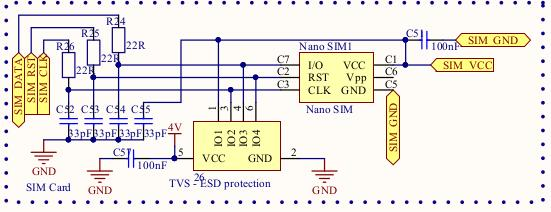
\includegraphics[width=15cm]{img/schematics/mainboard_gsm_sim_card.jpg}
	\caption{Schemat modułu karty SIM w urządzeniu lokalizującym}
	\label{fig:image_mainboard_functional_gsm_sim_card}
\end{figure}

\subsection{Moduł pamięci flash}

Wewnętrzna pamięć flash mikrokontrolera jest niewystarczająca, aby przechowywać w niej trasy wraz z parametrami jazdy. Stąd też pojawia się konieczność zastosowania zewnętrznego układu pamięci nieulotnej. Zastosowana w urządzeniu pamięć flash posiada pojemność 8 MB, co umożliwi przechowywanie wielu długich tras oraz dokładne profilowanie statystyczne stylu jazdy kierowcy. Schemat pamięci w urządzeniu lokalizującym pokazano na rysunku \ref{fig:image_mainboard_functional_flash}.

\begin{figure}[H]
	\centering
	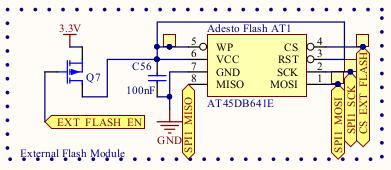
\includegraphics[width=15cm]{img/schematics/mainboard_functional_flash_memory.jpg}
	\caption{Schemat modułu pamięci flash w urządzeniu lokalizującym}
	\label{fig:image_mainboard_functional_flash}
\end{figure}

\subsection{Moduł akcelerometra}

Kolejną ważną częścią urządzenia jest moduł akcelerometru. Pozwala on na wybudzenie urządzenia w momencie przemieszczenia pojazdu, a w razie braku dezaktywacji - uruchomienie procedury alarmowej. Ponadto, dzięki jego wskazaniom możliwe jest wyznaczenie przyspieszenia pojazdu pozwalające na profilowanie stylu prowadzenia pojazdu przez kierowcę. Wbudowany żyroskop pozwoli na dokładniejsze profilowanie stylu jazdy kierowcy w trakcie pokonywania zakrętów oraz zmiany pasa.
Schemat modułu akcelerometra przedstawiono na rysunku \ref{fig:image_mainboard_functional_accelerometer}.


\subsection{Moduł NFC}

Moduł ten stanowi istotną część z punktu widzenia bezpieczeństwa komunikacji bezprzewodowej. Jest ono zapewnione poprzez zastosowanie szyfrowania wiadomości. Jeśli jednak ktoś podsłucha transmisję inicjalizacji urządzenia, w której przekazywane są klucze szyfrujące, cały koncept traci sens. Dzięki zastosowaniu modułu NFC, możliwość podsłuchania transmisji wymiany kluczy szyfrujących zostaje zniwelowana poprzez fizyczne ograniczenia zasięgu komunikacji. NFC posiada zasięg maksymalny do 5 cm.
Komunikacja odbywa się pomiędzy dwoma urządzeniami. Ze względu na sposób transmisji, jedno z urządzeń inicjuje komunikację. Inicjator generuje zmienne pole magnetyczne, w który może (lecz nie musi) zawrzeć dane wysyłane do urządzenia docelowego. Urządzenie docelowe wykrywa to pole i może odpowiedzieć poprzez odpowiednie zniekształcenie go, które jest wykrywane przez inicjator. Urządzenie docelowe nie generuje żadnego pola magnetycznego. Może jedynie zniekształcać pole generowane przez inicjator. Stąd wynika, że inicjator musi mieć znacznie większe zużycie energii niż urządzenie docelowe – tag. W urządzeniu lokalizacyjnym zastosowano moduł inicjatora NFC, którego schemat przedstawiono na rysunkach \ref{fig:image_mainboard_NFC_digital} - część cyfrowa oraz \ref{fig:image_mainboard_NFC_analog} - część analogowa.

\begin{figure}[H]
	\centering
	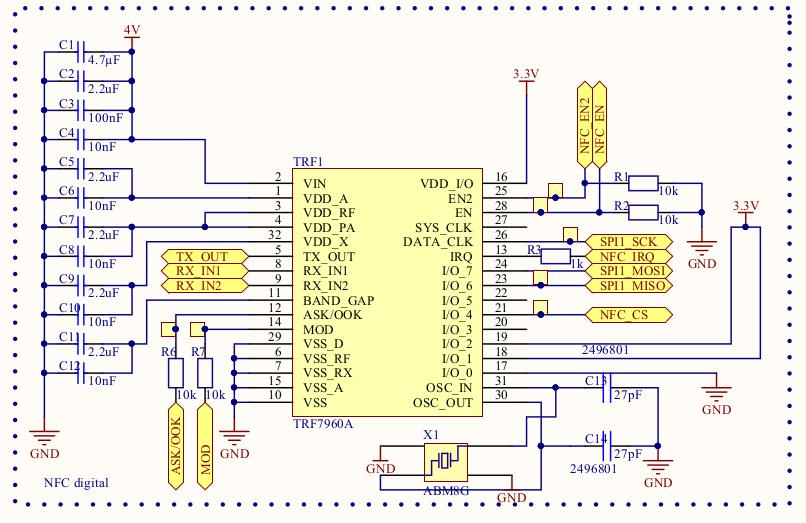
\includegraphics[width=15cm]{img/schematics/mainboard_NFC_chip.jpg}
	\caption{Schemat części cyfrowej modułu NFC w urządzeniu lokalizującym}
	\label{fig:image_mainboard_NFC_digital}
\end{figure}

\begin{figure}[H]
	\centering
	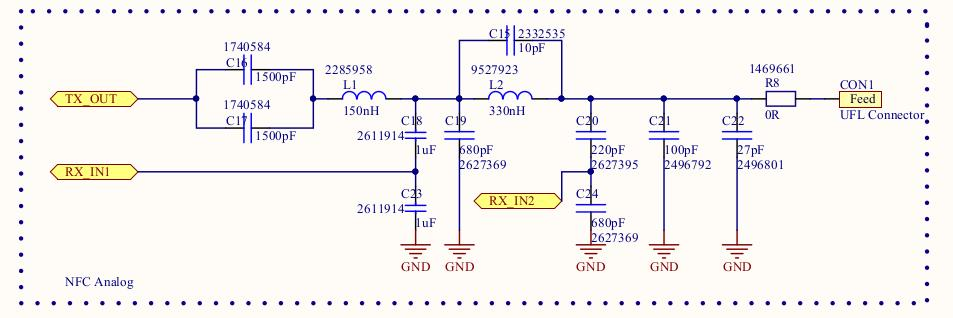
\includegraphics[width=15cm]{img/schematics/mainboard_NFC_analog.jpg}
	\caption{Schemat części analogowej modułu NFC w urządzeniu lokalizującym}
	\label{fig:image_mainboard_NFC_analog}
\end{figure}


\clearpage
\section{Urządzenie deaktywujące}

Głównym zadaniem tego urządzenia jest cykliczne rozgłaszanie swej obecności. Po wykryciu przez urządzenie lokalizujące, łączy się ona z deaktywatorem oraz bezpiecznym kanałem dokonywane jest wyłączenie funkcji alarmu. Dzięki temu, że urządzenie to ma tak proste zadanie, nie pobiera ona dużo poboru energii, więc możliwe jest zasilenie go ze standardowej baterii CR2032 o promieniu 20 mm i grubości 3.2 mm. Urządzenie to, przy odpowiedniej konfiguracji parametrów transmisji może działać kilka lat bez konieczności wymiany baterii. Zastosowanie wspomnianego źródła zasilania stanowi kompromis pomiędzy czasem działania i rozmiarem urządzenia, które docelowo powinno być umieszczone przy kluczach samochodowych. Schemat deaktywatora przedstawiono na rysunku \ref{fig:image_mainboard_NFC_schematic}.

\begin{figure}[h]
	\centering
	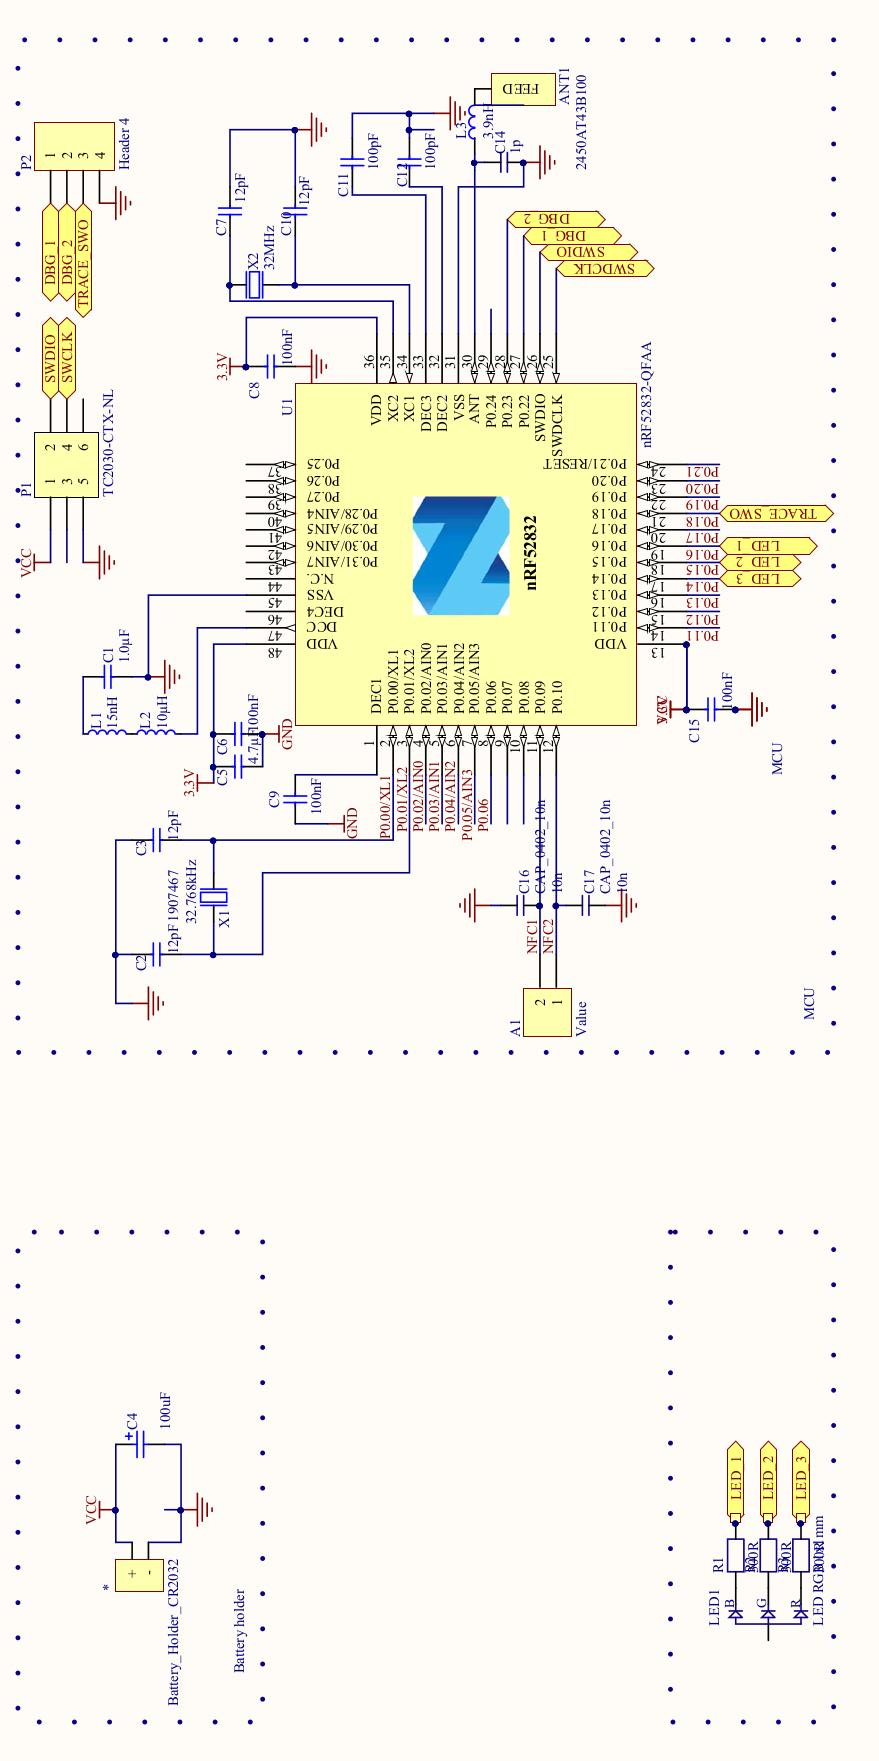
\includegraphics[width=12cm]{img/schematics/keytag.jpg}
	\caption{Schemat modułu zasilania urządzenia deaktywującego}
	\label{fig:image_keytag_schematic}
\end{figure}
